Naturalnym jest więc, że w praktyce często rozważamy modele wielowymiarowych zmiennych losowych, które mają regularne, łatwe do opisania gęstości łączne. Rozkłady jednowymiarowe z tabeli \ref{tab:przykladowe_zmienne_losowe} w naturalny sposób znajdują swoje rozszerzenia na więcej wymiarów (\cite{MultivariateDistributions}, \cite{Cherubini_Copula_Methods_in_Finance}). Najpopularniejszym tego przykładem jest rodzina $d$-wymiarowych rozkładów eliptycznych, do której należą rozkłady o gęstości postaci:

$$ f_{\mathcal{N}}(x, \mu, \Sigma) = k_d \vert\Sigma\vert^{-0.5}g\big((x-\mu)^T\Sigma^{-1}(x-\mu)\big).$$

W powyższej reprezentacji, $k_d \in\mathbb{R}$ jest stałą zależną od wymiaru, $\mu$ jest $d$-wymiarowym wektorem średnich, $\Sigma \in \mathbb{R}^{d \times d}$ to symetryczna, dodatnio zdefiniowana macierz, a $g \colon [0, \infty) \mapsto [0, \infty)$ jest pewną funkcją która nie zależy od wymiaru wektora.

Dla odpowiednio dobranych $g$ i $k_d$ otrzymamy w tej rodzinie wielowymiarowy rozkład normalny, czy wielowymiarowy rozkład t. Powstają one przy odpowiednio $k_d=(2\pi)^{-0.5d}$ i $g(s) = \exp(-0.5 t)$, lub $k_d=\Gamma(\frac{\nu + d}{2})/\Gamma(\frac{\nu}{2})$ i $g(s) = \big(1 + \frac{t}{\nu})^{-(\nu + d)/2}$.
\begin{figure}[H]
	\centering
	\includegraphics[width=0.45\linewidth]{01_MultivariateGaussian}	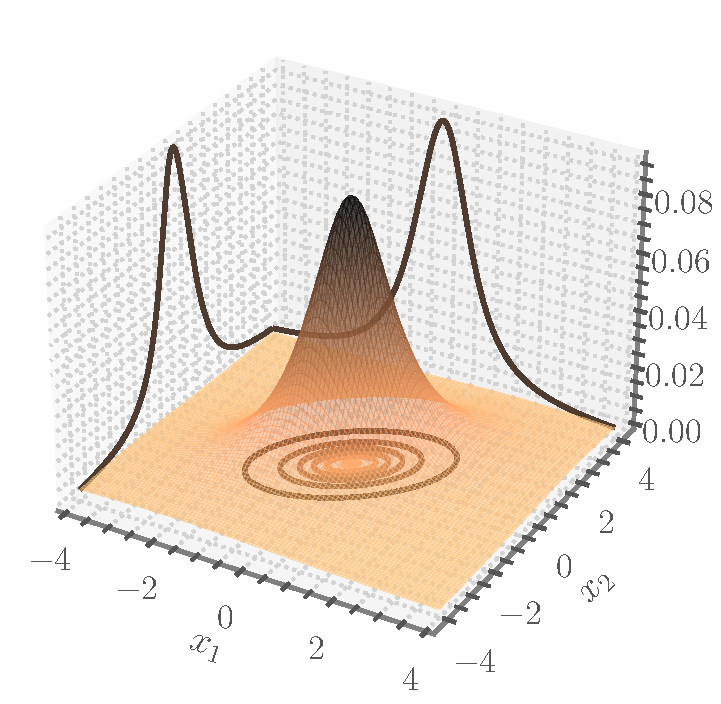
\includegraphics[width=0.45\linewidth]{01_MultivariateStudent}
	\caption{Gęstości przykładowych rozkładów eliptycznych ($d=2, \mu=[0, 0], \Sigma = \big[\begin{smallmatrix}2&1\\1&2\end{smallmatrix}\big]$). Lewy panel: $2$-wymiarowy rozkład normalny. Prawy panel: $2$-wymiarowy rozkład t ($\nu = 0.5$).\label{fig:multivariate_gaussian_student}}
\end{figure}

Używając rozkładów eliptycznych implikujemy model w którym rozkłady brzegowe pochodzą z tej samej rodziny. Obserwując rysunek \ref{fig:multivariate_gaussian_student}, można rozpoznać charakterystyczne kształty rozkładów brzegowych. Manipulując różnymi rozkładami eliptycznymi możemy więc zamodelować różne struktury korelacji między zmiennymi, czy też ciężkość ogonów, lecz tracimy swobodę wyboru rozkładów brzegowych. \cite{Markovitz_MPT} i jego model bazują właśnie na rozkładzie multinormalnym ponieważ zakładają, że wektor średnich i macierz korelacji wystarczająco opisuje rozkład zwrotów aktywów rynkowych. Podejście to łatwo obalić ze względu na empiryczne dowody ciężkoogonowego charakteru zachowania rynku akcji \cite{Mandelbrot_NonGaussianity}, czy zjawiska niesymetrycznej, silniejszej korelacji w lewym ogonie \cite{AssymetricEquityDependency}. Nie mniej jednak nie da się odmówić, że ten prosty model jest wystarczający aby uświadomić jak istotny jest wpływ zależności komponentów na zachowanie całego systemu.\\